\section{Results and Discussion}
\label{sec:results}

\subsection{Overall Top Models}

Hyperparameter searches are purely experimental and can be infinitely expanded. Through using the most often used hyperparameter values in LSC tasks, a foundation is made for where to begin. \autoref{fig:score-dist} shows the distribution of Spearman's $\rho$ scores for English, German, Latin, and Swedish respectively. The wide variations of scores for each language in these distributions demonstrate the lack of understanding in the effects of the interactions betwen hyperparameters on the overall performance of the models. Latin's score distribution in \autoref{fig:score-dist-lat} indicates that most of the models trained resulted in an average score. Without a hyperparameter search, there is a high chance that the model trained on Latin corpora will have an average score. Contrastively, the score distributions for English, German, and Swedish in  \autoref{fig:score-dist-eng}, \autoref{fig:score-dist-deu}, and \autoref{fig:score-dist-sve} respectively, indicate that hyperparameter searches are worth conducting. Majority of the 3 figures' model scores are low or average and the top-performing models only make up a small percentage of the total scores. More evident in \autoref{fig:score-dist-sve}, Swedish is at a higher risk of having a model that will perform poorly due do its incredibly large range of scores. A general analysis of the overall top-performing models for each language will be analysed in this section. Findings of the effects of each hyperparameter on the performance for each language will also be discussed below. 

\begin{figure}[h]
  \centering
  \subcaptionbox{\label{fig:score-dist-eng}English}{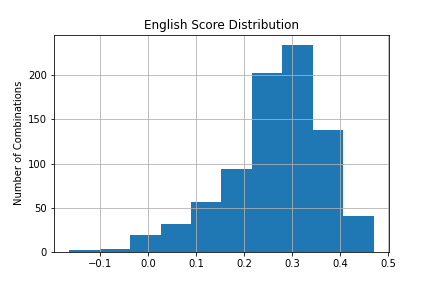
\includegraphics[width = 3in]{sections/figures/eng_score_distribution.png}}\quad
  \subcaptionbox{\label{fig:score-dist-deu}German}{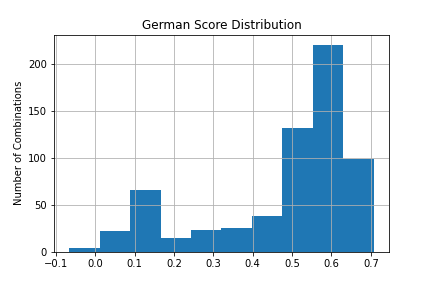
\includegraphics[width = 3in]{sections/figures/deu_score_distribution.png}}\\
  \subcaptionbox{\label{fig:score-dist-lat}Latin}{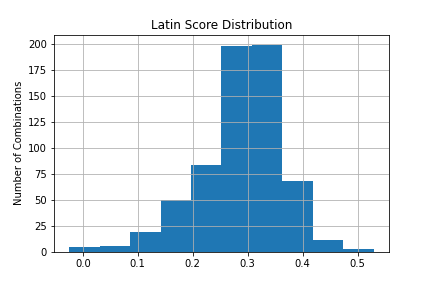
\includegraphics[width = 3in]{sections/figures/lat_score_distribution.png}}\quad
  \subcaptionbox{\label{fig:score-dist-sve}Swedish}{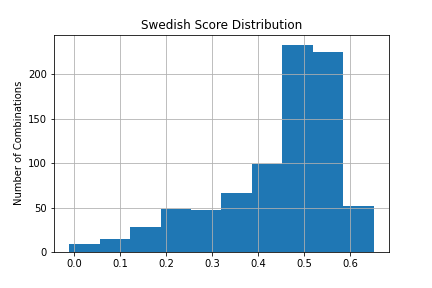
\includegraphics[width = 3in]{sections/figures/sve_score_distribution.png}}
  \caption{Distribution of Spearman's $\rho$ Scores for Each Language}
  \label{fig:score-dist}
\end{figure}


The hyperparameter search successfully found model combinations that outperformed both the best teams in the SemEval task and \citet{kaiser-etal-2020-ims}’s post-hoc optimizations for both English and Latin. As seen in \autoref{tab:performance-comparison}, a model was found to surpass the score of the best team in SemEval but not \citet{kaiser-etal-2020-ims} for the German language. The top-performing models for each language and their hyperparameters are shown in \autoref{tab:top-models}. Although it is important to analyse the top results for each language separately, it is also interesting to see commonalities between all four languages. The Orthogonal Procrustes alignment method seems to be the most effective for bigger datasets. For smaller datasets such as Latin, the Incremental Training alignment method is the most effective as the second time period model has information learned from both the first and second time period corpora. Epochs were also surprisingly low and lower frequency thresholds performed best as it included the maximum amount of words in the model’s vocabulary. Typically, longer epochs usually means more time for the model to learn more from the data and the nuances within that data. However, there is a certain threshold where the model stops learning what is useful and begins to learn noise which could lead to a decrease in model performance. 

\begin{table}
\centering
\begin{tabular}{|l|c|c|c|} 
\cline{2-4}
\multicolumn{1}{l|}{\textbf{ }} & \textbf{SemEval } & \textbf{Kaiser }         & \textbf{Best }            \\ 
\hline
English                         & \textit{ .422 }   & \textit{ .460 }          & \textbf{\textit{ .469 }}  \\ 
\hline
German                          & \textit{ .725 }   & \textit{\textbf{ .780 }} & \textit{ .706 }           \\ 
\hline
Latin                           & \textit{ .462 }   & \textit{ .410 }          & \textbf{\textit{ .529 }}  \\ 
\hline
Swedish                         & \textit{ .604 }   & \textit{\textbf{ .670 }} & \textit{ .651 }           \\
\hline
\end{tabular}
\caption{Top $\rho$ score comparison between SemEval-2020 Task 1 Subtask 2 teams, \citet{kaiser-etal-2020-ims}, and results.}
\label{tab:performance-comparison}
\end{table}


\begin{table}[h]
\centering
\begin{tabular}{cccccccc} 
\toprule
\textbf{ } & \textbf{ Algorithm } & \textbf{ Alignment } & \textbf{ Vocab Size } & \textbf{ Epochs } & \textbf{ Dims } & \textbf{ Freq Threshold } & \textbf{ $\rho$ }  \\
English    & FT              & OP               & ALL (16429)      & 5                 & 300             & 10               & .469            \\
German     & W2V             & OP               & ALL (218507)     & 5                 & 25              & 5                & .706            \\
Latin      & W2V             & INC              & -                & 5                 & 10              & 10               & .529            \\
Swedish    & FT              & OP               & 5000             & 10                & 50              & 10               & .651            \\
\bottomrule
\end{tabular}
\caption{Top-performing models for each language and their parameters. Abbreviations: W2V=Word2Vec, FT=FastText, OP=Orthogonal Procrustes, INC=Incremental.}
\label{tab:top-models}
\end{table}

The following analyses will show the differences in scores when the top-performing model is taken for each language and each hyperparameter is kept the same except for one hyperparameter. For example, Latin’s best model has the hyperparameters: Word2Vec, Incremental Training, 5 epochs, 10 dimensions, 10 frequency threshold. To explore the effects of the change in epochs, all the hyperparameters will remain the same except for epochs. The scores for each of these models are represented by a point in the graph where the $x$-axis is hyperparameter in question and the $y$-axis is  the Spearman's $\rho$ score. These points are joined by a dotted line graph and each line represents one of the four languages. Points that are in grey are statistically insignificant where p-value > 0.05 but they are included for informational purposes. Individual hyperparameter graphs for each language are available in \autoref{app-topmodelgraphs}. In order to extrapolate information from the data collected, the dotted lines are created in order to see trends between the points. However, it is acknowledged that if models were actually trained for each increase in the hyperparameter in question, there is a possibility that the trends would be different. 
%\cmtKV[inline]{should i write the last sentence to sound less invalidating (alternative phrase "trends in reality could show very different results."}

The relationship between epochs and performance raises the question of priority of performance and environmental impact. In \autoref{fig:all-epochs}, English and Swedish do not have 100-epoch models since it was deemed that their improved performance return was minimal compared to the time spent and energy consumption for training. There is a general decline in $\rho$ as epochs are increased for English, Latin, and Swedish while German had a slight increase in $\rho$ from 50 to 100 epochs. German and Latin appear to experience a similar decrease by 20 epochs but diverge after 50 epochs where German increases and Latin significantly decreases. As seen in \autoref{tab:subcorpora-size}, the German diachronic corpora has a total of 142.5 million tokens while the Latin diachronic corpora has 11.1 million tokens. This divergence might be attributed to the dataset size since the German corpora is much larger and there is more for the model to learn as epochs are increased.  On the other hand, the Latin corpora is very limited and after 50 epochs, the decrease in $\rho$ could be additional noise being introduced to the model. Although there might still be an increase in performance when training for more than 50 or 100 epochs, lower epochs seem to be the better choice for LSC. It also is a question of priority—smaller epochs or spending more time, memory, and energy. \cmtKV{is the last sentence more opinionated, should it be included, how could i word it to not sound as opinionated}For this hyperparameter, the option to have a smaller environmental impact compromises very little in terms of performance compared to the performance differences between lower epochs.  Environmental impact of longer training times for a slightly higher accuracy score is something that must be considered given the ongoing impacts of climate change on our planet. This consideration will be discussed further in Section~\ref{sec:ethicalcons}.

\begin{figure}[h]
  \centering
  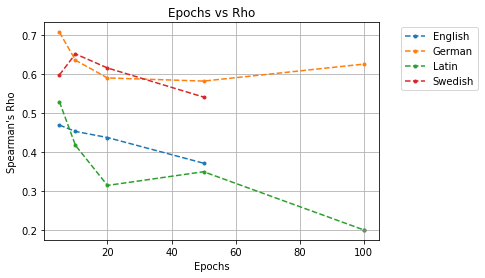
\includegraphics[width=.8\linewidth]{sections/figures/epochs_all.png}
  \caption{Change in Epochs vs. Score}
  \label{fig:all-epochs}
\end{figure}

The dimensions hyperparameter refers to the size of the vector for each word representation. Increasing vector dimensions requires a higher computational time and more memory. As expected, English performs best with higher dimensions. The 300-dimension hyperparameter is commonly in NLP tasks\cmtKV{should i cite something here or is this okay to just say} and is usually the baseline when conducting NLP (including LSC) tasks on other languages due to the prevalence in studies being done in English. As seen in \autoref{fig:all-dims}, choosing higher dimensions does not necessarily result in better $\rho$ scores as it does with the English language. German, Swedish, and Latin all have higher $\rho$ scores when lower dimensions are used. Latin’s top model performed best with the lowest dimension of 10. Since the Latin corpora is very small compared to the other three languages, having less abstractions of words in the vector representations might have been more useful for the model and minimised the introduction of noise. The genre makeup of corpora is also put into question as it seems to have an effect on the vector dimensions consequently affecting performance. Swedish and German are both composed of newspaper corpora and so the same style and type of language is used. English has a mixed genre corpora and Latin is somewhere in between. Since Swedish and German models are trained on texts that have their own writing style where constructions of sentences are similar but the words have been used under many contexts, vectors with higher dimensions allow for those nuances to be learned. On the other hand, the Latin corpora consists of a wide range of texts compiled and vectors with lower dimensions allow the model to learn the usages of the words in a broader context. The genres of text being included in the corpora must be taken into consideration before choosing the vector dimensions for a model. The typical baseline of 300 dimensions, based on English results in past NLP tasks, also shows not as effective on other languages.

\begin{figure}[h]
  \centering
  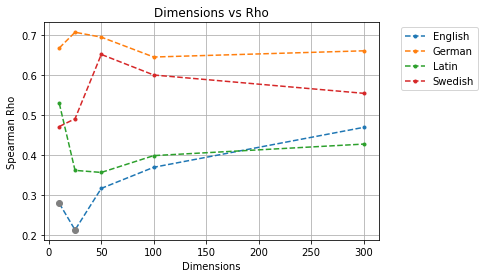
\includegraphics[width=.8\linewidth]{sections/figures/dims_all.png}
  \caption{Change in Dimensions vs. Score}
  \label{fig:all-dims}
\end{figure}

The frequency threshold hyperparameter refers to the minimum number of times a word has to appear in a corpus to be included in the model’s vocabulary. Smaller frequency thresholds will result in a larger vocabulary. Since the vocabulary is larger, memory needed will also be larger as there are more vectors to be stored and learned by the model.  \autoref{fig:all-freqs} illustrates that it is generally better to have a lower frequency threshold in order to ensure that majority of the words in a corpus is being included. German and Swedish do not have 4 points in \autoref{fig:all-freqs} as the $\rho$ scores for those model combinations were NaNs. While German performs best with the lowest frequency threshold of 5, English, Latin, and Swedish all perform better at a slightly higher frequency threshold of 10. Depending on the corpus being used, better performance with a higher frequency threshold could mean an effective filtering out of words that are seldom used in the corpus and do not effectively contribute to the target word's contextual meaning. A steady decrease in $\rho$ scores are seen as the frequency threshold increases. This is expected since a higher frequency threshold results in less words in the vocabulary and a smaller vocabulary naturally excludes words that contribute to the contextual meaning of a word. 

\begin{figure}[h]
  \centering
  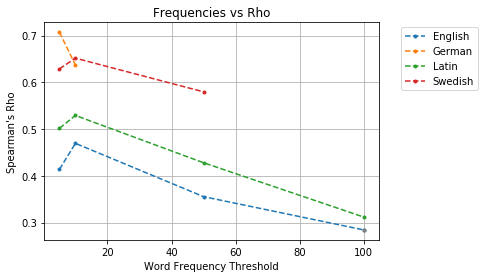
\includegraphics[width=.8\linewidth]{sections/figures/freqs_all.png}
  \caption{Change in Frequency Thresholds vs. Score}
  \label{fig:all-freqs}
\end{figure}

Two approaches were used for the Orthogonal Procrustes alignment method—Ryan Heuser’s Tutorial\footnote{\url{https://gist.github.com/quadrismegistus/09a93e219a6ffc4f216fb85235535faf}} and VecMap\footnote{\url{https://github.com/artetxem/vecmap}}. The former had a default of including the entire shared vocabulary of the first time period corpus and the second time period corpus during the alignment process. However, the latter included the option to indicate the size of the shared vocabulary during the alignment process. \autoref{fig:all-vocabalign} shows the effect of vocabulary size during the Orthogonal Procrustes alignment process on $\rho$ scores when using VecMap. Latin is not included in this graph since its top-performing model used the Incremental Training alignment method. English and German seem to be affected similarly from this hyperparameter while Swedish experiences the opposite. German profits when the entire vocabulary (where the shared vocabulary size is 218,507) is included in the alignment process and results in the top-performing model. Swedish experiences a similar increase in performance when the shared vocabulary size is 5000. However, the top-performing model for Swedish has a vocabulary size of 5000 and an increase in vocabulary size shows a decrease in $\rho$ scores. Although English has a significantly smaller corpora size, it also profits from the inclusion of the entire vocabulary (where the shared vocabulary size is 16,429) when aligning both time period models. \autoref{fig:all-vocabalign} shows that the most effective shared vocabulary size when using the Orthogonal Procrustes alignment method is language-specific and cannot be generalised. It also demonstrates the advantages of performing hyperparameter searches and that findings in one language are not always universal.

\begin{figure}[h]
  \centering
  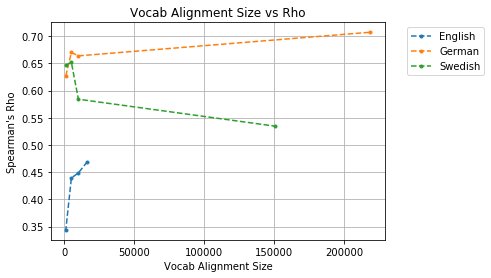
\includegraphics[width=.8\linewidth]{sections/figures/vocabalignment_all.png}
  \caption{Shared Vocabulary Size in Orthogonal Procrustes Alignment vs. Score}
  \label{fig:all-vocabalign}
\end{figure}

The results from this large-scale hyperparameter search introduces and substantiates some intuitions when selecting hyperparameters for future LSC tasks. There is a threshold for the amount of improvement in scores when models are trained with higher epochs. Models trained with generally lower epochs performed the best within the range chosen for this hyperparameter search. The standard of 300 dimensions as a baseline for vector representations, based on LSC tasks for the English language, does not necessarily apply to all languages. All 3 non-English languages in this task performed best with models that had lower dimensions. When choosing the dimensions of vectors, it is also important to consider the size of the corpora and the genres of texts included in the corpora. Larger corpora where the usage of words fall under the same writing style might need higher dimensions in order to learn the nuances whenever a word is used. Conversely, corpora smaller in size consisting of texts of a wider genre range would need lower dimensions in order to learn the usages of words in a broader context. In terms of frequency thresholds, a lower frequency threshold maximises the amount of words included in the vocabulary and this results in more contributions to the contextual meaning of each word. However, a slightly higher frequency threshold can be effective in filtering out words that are rarely used and do not contribute to the meaning of the target words. For models that perform better using the Orthogonal Procrustes alignment method, the size of the shared vocabulary during the aligning process can greatly affect the performance. Both English and German profit from including the entire shared vocabulary while Swedish performs better with a smaller shared vocabulary.

\subsection{Top Models Based on POS-Tag}

Every model trained was also evaluated by creating smaller target word lists based on each target word’s POS-tag. For each language’s target word list, the words have been manually annotated\footnote{Thank you to Barbara McGillivray, Konstantinos Mavromatakis, Merle Pfau, and Saga Hansson for manually annotating the Latin, German, and Swedish target word lists.} and POS-tagged as either a noun (nn), verb (vb), or adjective (adj). The target word list breakdown for each language is seen in \autoref{fig:target-postags}. Nouns are much more prevalent in the target word lists and so conclusions made for nouns are better grounded compared to conclusions made for verbs and adjectives. Control words within each POS-tag are indicated through a lighter colour respective of its POS-tag and offsetted in \autoref{fig:target-postags}. With already a smaller ratio and an addition of control words that have 0 as a cosine distance, a $\rho$ score of 1 can sometimes be more easily attained since it is calculated by rank. For example, \autoref{fig:postag-deu} shows that there are only 2 German target words that are adjectives and one is a control word. A model’s chances of obtaining a perfect Spearman's $\rho$ score of 1 is very high since the control word's cosine distance would be zero—making it very likely to have the correct ranking. 

%\cmtSH[inline]{Could you perhaps try to stick "the block of the same colour" together in the figure? Eg in Swedish and German. It's currently also difficult to know eg if the values for "nn" include those for "nn-control"}
%\cmtKV[inline]{REARRANGE PIE SLICES}
%\cmtSH{It would be wiser to rename, in the plot itself, "nn" to "nn-change" -- otherwise it's unclear whether nn-control is part of nn without doing the addition} 

\begin{figure}[h]
  \centering
  \vspace*{-2mm}
  \subcaptionbox{\label{fig:postag-eng}English (89$\%$ nouns, 11$\%$ verbs)}{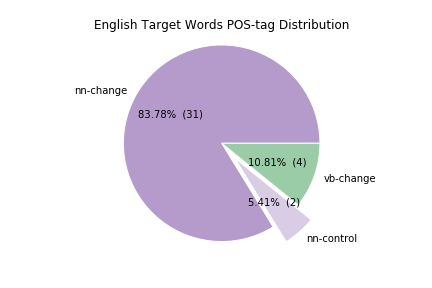
\includegraphics[width = 3in]{sections/figures/eng-pos-target-control.png}}\quad
  \subcaptionbox{\label{fig:postag-deu}German(67$\%$ nouns, 29$\%$  verbs, 4$\%$ adjectives)}{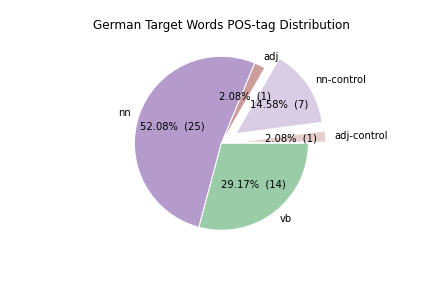
\includegraphics[width = 3in]{sections/figures/deu-pos-target-control.png}}\\
  \subcaptionbox{\label{fig:postag-lat}Latin (70$\%$ nouns, 12.5$\%$  verbs, 17.5$\%$ adjectives)}{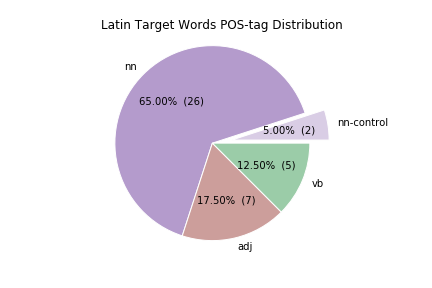
\includegraphics[width = 3in]{sections/figures/lat-pos-target-control.png}}\quad
  \subcaptionbox{\label{fig:postag-sve}Swedish (71$\%$ nouns, 19$\%$ verbs, 10$\%$ adjectives)}{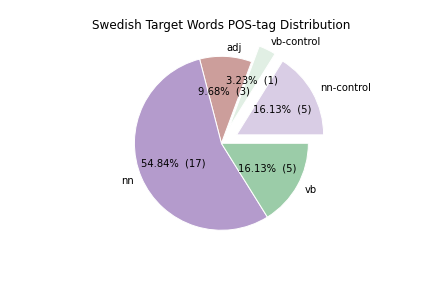
\includegraphics[width = 3in]{sections/figures/sve-pos-target-control.png}}
  \caption{Target Word POS-tag Distribution for Each Language. Control words (words that have not undergone semantic change) are shown through a lighter colour respective of its POS-tag and offsetted. Percentages are rounded to the nearest integer for readability.}
  \label{fig:target-postags}
\end{figure}

The tables below (\autoref{tab:eng-posresults}, \autoref{tab:deu-posresults}, \autoref{tab:lat-posresults}, \autoref{tab:sve-posresults}) for each language show the top-performing models based on the smaller target word lists created by sorting the target words by POS-tag. For each table, the first row is the overall top-performing model (entire target word list), included for easier comparisons to models that performed well detecting LSC for specific POS-tags. 

In the per POS-tag evaluation of models for English seen in \autoref{tab:eng-posresults}, it was interesting to see that every top-performing model, including the overall top-performing model, had the dimensions hyperparameter at 300. For all the POS-tag evaluations, higher epochs seem to have helped with increasing the $\rho$ score. However, it is important to keep in mind that there are only 4 verbs out of the 33 English target words. Since nouns makeup over 87\% of the English target word list, it makes sense that the top-performing model for nouns has a very similar hyperparameter combination as well as $\rho$ score. There is no top-performing model for adjectives since the English target word list did not have any adjectives. 


Word2Vec is prevalent in the German per POS-tag evaluation of models. As seen in \autoref{tab:deu-posresults}, there were 670 hyperparameter combinations that all obtained the perfect $\rho$ score of 1. There are only 2 adjectives out of 48 German target words and 1 adjective was a control word (where its cosine distance was 0). With this in mind, there is a higher chance that models would obtain a $\rho$ score of 1 since it is calculated through ranking. On the other hand, verbs makeup 29\% of the target words and the top-performing model scored quite well with only a $\Delta$ of 0.096. Overall, smaller dimensions result in better scores for the German target word list. 


The POS-tag evaluation of models for Latin seen in \autoref{tab:lat-posresults} had the greatest differences in hyperparameters compared to its overall top-performing model. All of the top-performing models for each POS-tag also had higher $\rho$ scores. All of the top-performing models for adjectives had Orthogonal Procrustes as the alignment method and surprisingly much higher epochs, dimensions, and frequencies—most being 50 epochs, 25 dimensions, and 100 frequency threshold. The high frequency threshold might be due to the high frequency (MUST CHECK VIA USAGES) of adjectives within the corpora. Majority of the words would have been then filtered out leaving a higher chance of very few words being left including the adjectives. The top-performing model for nouns had a higher $\rho$ score by a $\Delta$ of 0.174 but shares the same hyperparameters as the overall top-performing model except for the algorithm (FastText instead of Word2Vec) and a higher frequency threshold. Top-performing models for verbs (making up 12.5\% of the target words) tend to get better results with lower frequency thresholds.


Top-performing models for Swedish based on target word POS-tags seen in \autoref{tab:sve-posresults} were a bit scattered but still had commonalities. The most common for all POS-tag evaluations were 50 epochs, 100 dimensions, and 10 frequency threshold. Only the top-performing model for adjectives performed better than the overall top-performing model scoring a $\rho$ of 1 by a $\Delta$ of 0.349. However, there are only 3 adjectives out of the 31 Swedish target words. All of the top-performing models for verbs and nouns along with one of the top-performing models for adjectives have Incremental Training as the alignment method (contrasting the overall top-performing which has Orthogonal Procrustes) indicating that Incremental Training must learn something specific when it comes to detecting LSC for Swedish POS-tags. 

% bad conduct
\bigskip
\bigskip

\begin{table}[h]
\centering
\begin{tabular}{cccccccccc} 
\toprule
\textbf{ Algo } & \textbf{ Align } & \textbf{ Vocab Size } & \textbf{ Epochs } & \textbf{ Dims } & \textbf{ Freq} & \textbf{ Lg } & \textbf{ POS } & \textbf{ Rho } & \textbf{ $\Delta$ }  \\
FT              & OP               & ALL (16429)           & 5                 & 300             & 10             & ENG           & -              & .469           & -               \\
-               & -                & -                     & -                 & -               & -              & ENG           & ADJ            & -              & -               \\
FT              & INC              & -                     & 10                & 300             & 10             & ENG           & NN             & .463           & -0.005            \\
FT              & INC              & -                     & 50                & 300             & 5              & ENG           & VB             & .800           & +0.331            \\
FT              & INC              & -                     & 50                & 300             & 50             & ENG           & VB             & .800           & +0.331            \\
W2V             & OP               & -                     & 50                & 300             & 100            & ENG           & VB             & .800           & +0.331            \\
W2V             & OP               & 1000                  & 20                & 300             & 10             & ENG           & VB             & .800           & +0.331            \\
W2V             & OP               & 1000                  & 50                & 300             & 100            & ENG           & VB             & .800           & +0.331            \\
W2V             & OP               & 10000                 & 20                & 300             & 10             & ENG           & VB             & .800           & +0.331            \\
\bottomrule
\end{tabular}
\caption{English Top-performing Models for Each POS-tag}
\label{tab:eng-posresults}
\end{table}


%** WHERE IS THE MISSING DOLLAR SIGN\cmtSH{This was $^*$  for MODELS, fixed now -- the circonflex needs math mode to mean "to the x power"}
\begin{table}[h]
\centering
\begin{tabular}{cccccccccc} 
\toprule
\textbf{ Algo } & \textbf{ Align } & \textbf{ Vocab Size } & \textbf{ Epochs } & \textbf{ Dims } & \textbf{ Freq } & \textbf{ Lg } & \textbf{ POS } & \textbf{ Rho } & \textbf{ $\Delta$ }  \\
W2V             & OP               & ALL (218507)          & 5                 & 25              & 5              & DEU           & -              & .706           & -               \\
670             & MODELS$^*$       & GOT                   & SAME              & SCORE           & FOR            & DEU           & ADJ            & 1.00           & +0.294          \\
W2V             & INC              & -                     & 20                & 10              & 10             & DEU           & NN             & .187 (p=0.30)  & -0.518          \\
W2V             & INC              & -                     & 5                 & 50              & 5              & DEU           & VB             & .609           & -0.096          \\
\bottomrule
\end{tabular}
\caption{German Top-performing Models for Each POS-tag. $^*$670 models had a Spearman's $\rho$ score of 1. Please refer to the POS-tag results file available in \autoref{app-resources}.}
\label{tab:deu-posresults}
\end{table}


\begin{table}[h]
\centering
\begin{tabular}{cccccccccc} 
\toprule
\textbf{ Algo } & \textbf{ Align } & \textbf{ Vocab Size } & \textbf{ Epochs } & \textbf{ Dims } & \textbf{ Freq } & \textbf{ Lg } & \textbf{ POS } & \textbf{ Rho } & \textbf{ $\Delta$ }  \\
W2V             & INC              & -                     & 5                 & 10              & 10             & LAT           & -              & .529           & -               \\
W2V             & OP               & 1000                  & 50                & 25              & 100            & LAT           & ADJ            & .821           & +0.291          \\
FT              & OP               & 5000                  & 50                & 25              & 100            & LAT           & ADJ            & .821           & +0.291          \\
FT              & OP               & 10000                 & 50                & 25              & 100            & LAT           & ADJ            & .821           & +0.291          \\
FT              & OP               & ALL (1911)            & 50                & 25              & 100            & LAT           & ADJ            & .821           & +0.291          \\
FT              & INC              & -                     & 10                & 10              & 100            & LAT           & ADJ            & .821           & +0.291          \\
FT              & INC              & -                     & 20                & 25              & 100            & LAT           & ADJ            & .821           & +0.291          \\
FT              & INC              & -                     & 5                 & 10              & 50             & LAT           & NN             & .704           & +0.174          \\
W2V             & INC              & -                     & 5                 & 25              & 10             & LAT           & VB             & 1.0            & +0.471          \\
W2V             & INC              & -                     & 5                 & 100             & 10             & LAT           & VB             & 1.0            & +0.471          \\
W2V             & INC              & -                     & 5                 & 300             & 5              & LAT           & VB             & 1.0            & +0.471          \\
W2V             & INC              & -                     & 5                 & 300             & 10             & LAT           & VB             & 1.0            & +0.471          \\
W2V             & INC              & -                     & 10                & 100             & 5              & LAT           & VB             & 1.0            & +0.471          \\
W2V             & INC              & -                     & 10                & 300             & 10             & LAT           & VB             & 1.0            & +0.471          \\
W2V             & INC              & -                     & 20                & 300             & 10             & LAT           & VB             & 1.0            & +0.471          \\
W2V             & INC              & -                     & 50                & 300             & 10             & LAT           & VB             & 1.0            & +0.471          \\
W2V             & INC              & -                     & 100               & 300             & 10             & LAT           & VB             & 1.0            & +0.471          \\
FT              & INC              & -                     & 20                & 100             & 10             & LAT           & VB             & 1.0            & +0.471          \\
FT              & INC              & -                     & 20                & 300             & 5              & LAT           & VB             & 1.0            & +0.471          \\
FT              & INC              & -                     & 50                & 100             & 5              & LAT           & VB             & 1.0            & +0.471          \\
\bottomrule
\end{tabular}
\caption{Latin Top-performing Models for Each POS-tag}
\label{tab:lat-posresults}
\end{table}


\begin{table}[h]
\centering
\begin{tabular}{cccccccccc} 
\toprule
\textbf{ Algo } & \textbf{ Align } & \textbf{ Vocab Size } & \textbf{ Epochs } & \textbf{ Dims } & \textbf{ Freq } & \textbf{ Lg } & \textbf{ POS } & \textbf{ Rho } & \textbf{ $\Delta$ }  \\
FT              & OP               & 5000                  & 10                & 50              & 10                        & SVE           & -              & .651           & -               \\
FT              & OP               & 1000                  & 50                & 100             & 50                        & SVE           & ADJ            & 1.0            & +0.349          \\
FT              & INC              & -                     & 50                & 300             & 50                        & SVE           & ADJ            & 1.0            & +0.349          \\
W2V             & OP               & 1000                  & 50                & 100             & 50                        & SVE           & ADJ            & 1.0            & +0.349          \\
W2V             & OP               & 5000                  & 20                & 300             & 10                        & SVE           & ADJ            & 1.0            & +0.349          \\
W2V             & OP               & -                     & 10                & 100             & 10                        & SVE           & ADJ            & 1.0            & +0.349          \\
W2V             & INC              & -                     & 20                & 10              & 10                        & SVE           & NN             & .464           & -0.187          \\
FT              & INC              & -                     & 50                & 100             & 100                       & SVE           & VB             & .371           & -0.280          \\
W2V             & INC              & -                     & 20                & 10              & 10                        & SVE           & VB             & .371           & -0.280          \\
W2V             & INC              & -                     & 50                & 10              & 5                         & SVE           & VB             & .371           & -0.280          \\
\bottomrule
\end{tabular}
\caption{Swedish Top-performing Models for Each POS-tag}
\label{tab:sve-posresults}
\end{table}

% this is probably bad conduct
\bigskip
\bigskip
\bigskip
\bigskip
POS-tag evaluation of all the models trained shows that there are hyperparameter combinations that perform better when detecting LSC for specific POS-tags than the overall top-performing model. It also shows that some hyperparameter combinations can be used in order to better detect LSC depending on the target words’ POS-tag. 
